% !TEX encoding = UTF-8 Unicode
%!TEX TS-program = xelatex

\documentclass[12pt]{extarticle}
% extarticle is like article but can handle 8pt, 9pt, 10pt, 11pt, 12pt, 14pt, 17pt, and 20pt text

\def \ititle {Origins of Mind}
 
\def \isubtitle {Lecture 08}
 
\def \iauthor {Stephen A. Butterfill}
\def \iemail{s.butterfill@warwick.ac.uk}
\date{}

%for strikethrough
\usepackage[normalem]{ulem}

\usepackage{pdfpages}

\usepackage{fitch}


\input{$HOME/Documents/submissions/preamble_steve_handout}

%logic symbol \leftmodels
\usepackage{MnSymbol}

%\bibpunct{}{}{,}{s}{}{,}  %use superscript TICS style bib
%remove hanging indent for TICS style bib
%TODO doesnt work
\setlength{\bibhang}{0em}
%\setlength{\bibsep}{0.5em}


%itemize bullet should be dash
\renewcommand{\labelitemi}{$-$}

\begin{document}

%\raggedcolumns

\begin{multicols*}{3}

\setlength\footnotesep{1em}


\bibliographystyle{newapa} %apalike

%\maketitle
%\tableofcontents




%--------------- 
%--- start paste
\def \ititle {Logic I}
 
\def \isubtitle {Lecture 17}
 
\begin{center}
 
{\Large
 
\textbf{\ititle}: \isubtitle
 
}
 
 
 
\iemail %
 
\end{center}
 
Readings refer to sections of the course textbook, \emph{Language, Proof and Logic}.
 
 
 
\section{Revison: Definitions}
 
\emph{Exercise} State the rules of proof for the following two connectives: ∧ →
 
What is a logically valid argument?
 
What is ... logical consequence, a tautology, a contradiction, a counterexample, a subproof, ...
 
What is a proof?
 
 
 
\section{Revison: Truth tables}
 
Use truth tables to establish whether the following arguments are valid. If any arguments are invalid, state counterexamples to them. If any arguments are valid, explain carefully using the truth tables why they are valid.
 
\begin{enumerate}
 
\item
 
\begin{equation*}
\begin{fitch}
\fh P \to Q \\
\fa \lnot P \lor Q \\
\end{fitch}
\end{equation*}
 
\item
 
\begin{equation*}
\begin{fitch}
\fh P ↔ (Q \to Q) \\
\fa P \lor Q \\
\end{fitch}
\end{equation*}
 
\item
 
\begin{equation*}
\begin{fitch}
\fh P \lor \lnot(Q \land R) \\
\fa P \lor (\lnot Q \land R) \\
\end{fitch}
\end{equation*}
 
\end{enumerate}
 
 
 
\section{Revison: Proofs (propositional)}
 
\begin{enumerate}
 
\item
 
\begin{equation*}
\begin{fitch}
\fh \lnot P \land R \\
\fa \lnot P \\
\end{fitch}
\end{equation*}
 
\item
 
\begin{equation*}
\begin{fitch}
\fh \lnot P \lor R \\
\fa P \to R \\
\end{fitch}
\end{equation*}
 
\end{enumerate}
 
 
 
\section{Revison: Proofs (with quantifiers)}
 
\begin{enumerate}
 
\item
 
\begin{equation*}
\begin{fitch}
\fh ∀x S(x) \\
\fh ∀x \lnot S(x) \\
\fa $\bot$ \\
\end{fitch}
\end{equation*}
 
\item
 
\begin{equation*}
\begin{fitch}
\fh ∀x ( F(x) → x=a ) \\
\fa ¬∃x ( F(x) ∧ ¬x=a ) \\
\end{fitch}
\end{equation*}
 
\item
 
\begin{equation*}
\begin{fitch}
\fh ∃x ∀y ( F(y) → ¬G(x,y) ) \\
\fa ∀y ∃x ( F(y) → ¬G(x,y) ) \\
\end{fitch}
\end{equation*}
 
\end{enumerate}
 
 
 
\section{Revison: Translation from English to FOL}
 
\emph{Exercise} Translate the following sentences of English into FOL using the interpretation below:
 
\hspace{5mm} L(x,y)	: x is a logical consequence of y
 
\hspace{5mm} N(x,y)	: x is the negation of y
 
\hspace{5mm} S(x)	: x is a sentence
 
\hspace{5mm} a	 : ‘Fire melts ice’
 
i.	‘Fire melts ice’ is a sentence
 
ii.	There is a sentence
 
iii.	There is a sentence which is the negation of ‘Fire melts ice’
 
iv.	Some sentences are contradictions and all contradictions are logically equivalent.
 
 
 
\section{Does ‘if’ mean what ‘→’ means?}
 
\emph{Reading:} §7.3
 
\begin{minipage}{\columnwidth}
 
These two arguments are valid: does that mean that `if' means what `→' means?
 
\begin{center}
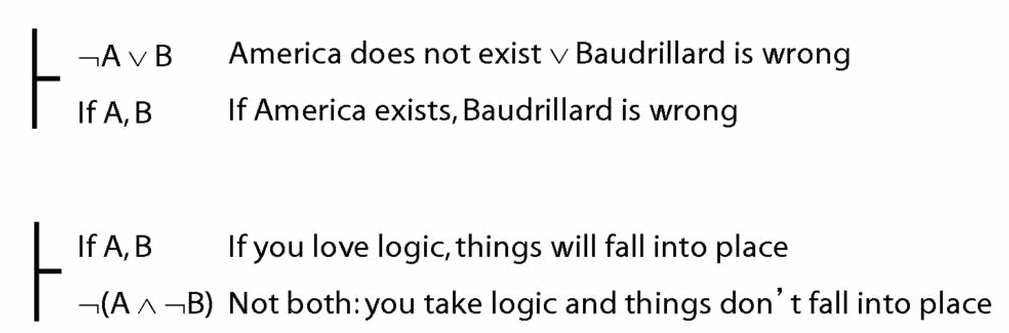
\includegraphics[scale=0.3]{img/if_is_arrow.png}
\end{center}
\end{minipage}
 
\begin{minipage}{\columnwidth}
 
The English argument isn't valid; the FOL argument is valid; therefore `if' can't mean what `→' means?
 
\begin{center}
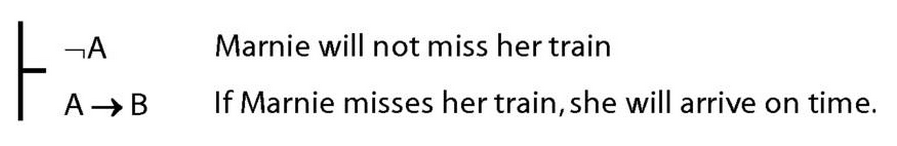
\includegraphics[scale=0.3]{img/if_aint_arrow.png}
\end{center}
\end{minipage}
 
 
 
\section{Proof Example: ∃x Dead(x) $\vdash$ ¬∀x¬ Dead(x).}
 
\begin{center}
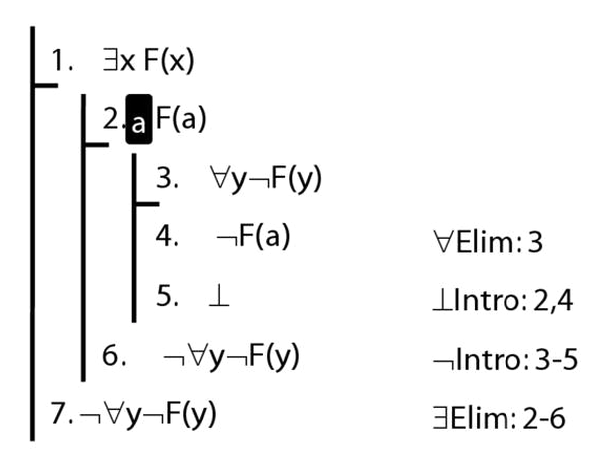
\includegraphics[scale=0.3]{img/unit_825_proof.png}
\end{center}
 
 
\section{Proof Example: ¬∀x Dead(x) $\vdash$ ∃x¬ Dead(x).}
 
\begin{center}
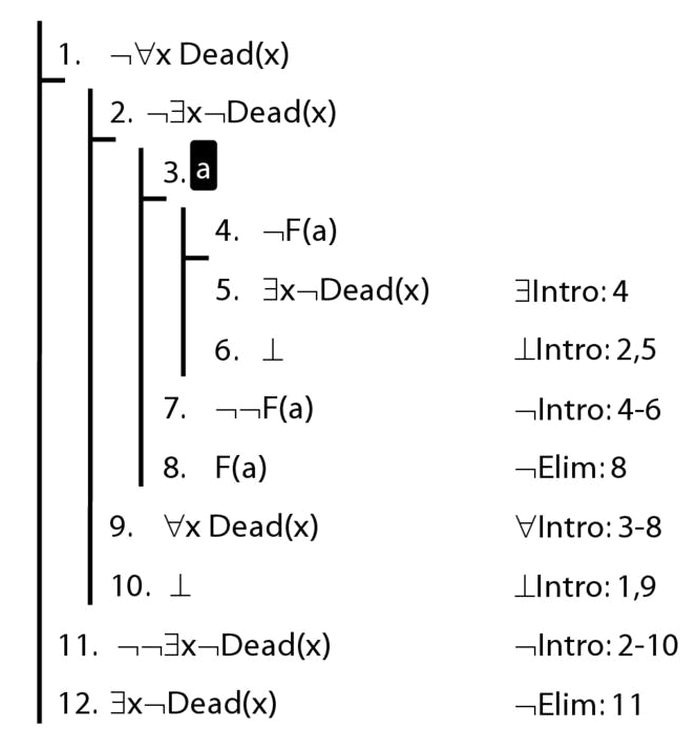
\includegraphics[scale=0.3]{img/unit_826_proof.png}
\end{center}
 
  
 
 
\section{The End Is Near}
 
\emph{Reading:} §14.3
 
‘The’ can be a quantifier, e.g. ‘the square is broken’. How to formalise it?
 
The square is broken
 
$\leftmodels\models$ There is exactly one square and it is broken
 
$\leftmodels\models$ There is at most one square and there is at least one square and it is broken
 
$\leftmodels\models$ There is at most one square and there is at least one square and all squares are broken
 
$\leftmodels\models$ ¬ ∃x ∃y ( Square(x) ∧ Square(y) ∧ ¬x=y )
 
\hspace{5mm} ∧ ∃x Square(x)
 
\hspace{5mm} ∧ ∀x ( Square(x) → Broken(x) )
 
Which shorter sentences are equivalent to this?
 
∃x ( Square(x) ∧ ∀y ( Square(y) → y=x ) ∧ Broken(x) )
 
∃x ( ∀y ( Square(y) ↔ y=x ) ∧ Broken(x) )
 
%--- end paste
%--------------- 
 


\end{multicols*}

\end{document}